\chapter{Analisis}
\label{chap:analisis}
Pada bab ini dijelaskan mengenai analisis aplikasi pengiriman data pada WSN, analisis proses pengiriman data dari node sensor ke \textit{base station} pada WSN, dan analisis terhadap protokol transfer yang \textit{reliable} pada \textit{Wireless Sensor Network}.

\section{Analisis Aplikasi Pengiriman Data Pada WSN}
Aplikasi transfer data pada WSN dapat menggunakan arsitektur flat maupun hierarki. Komunikasi yang dilakukan pada setiap arsitektur dapat menggunakan \textit{single-hop} maupun \textit{multi-hop}. Dalam melakukan transfer data dapat terjadi \textit{loss}. Untuk menangani \textit{loss} harus dilakukan pengiriman ulang data atau \textit{retransmission}.

Pada skripsi ini dibangun aplikasi yang dapat melakukan transfer data dari node sensor ke \textit{base station}. Aplikasi WSN yang dibangun menggunakan arsitertur flat dengan \textit{single-hop} dan \textit{multi-hop}. Aplikasi ini digunakan untuk mengetahui keadaan suatu tempat atau daerah dengan bantuan node sensor untuk mendapatkan data (\textit{sensing}). 

Aplikasi ini memiliki beberapa fungsi. Fungsi utama pada aplikasi ini adalah untuk melakukan transfer data dari setiap node sensor. Fungsi lain pada aplikasi ini dijelaskan menggunakan diagram \textit{use case} pada Gambar~\ref{fig:usecase} dan skenario pada Tabel~\ref{tab:skenario1} sampai Tabel~\ref{tab:skenario6}.

\begin{figure}[H]
	\centering
	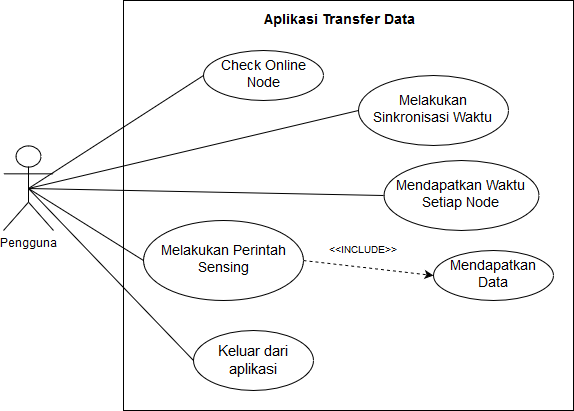
\includegraphics[scale=0.7]{usecase}
	\caption{Diagram \textit{use case} aplikasi data transfer pada WSN}
	\label{fig:usecase}
\end{figure}

\begin{table}[H]
    \centering
    \caption{Tabel skenario Check Online Node.}
    \begin{tabular}{|p{3cm}|p{10cm}|}
    \hline
        Nama & Check Online Node\\
    \hline
    \hline
        Deskripsi & Mengetahui node-node mana saja yang sedang menyala (\textit{online}). \\
    \hline
        Aktor & Pengguna \\
    \hline
        Pre-kondisi & Menjalankan aplikasi \\
    \hline
        Alur Skenario Utama & 
        \begin{enumerate}
            \item Sistem memuat aplikasi.
            \item Sistem menampilkan pilihan untuk dipilih pengguna.
            \item Pengguna memilih "Check Online Node".
            \item Sistem menampilkan semua node yang sedang menyala (\textit{online}).
            \item Sistem kembali pada tampilan utama.
        \end{enumerate}\\
    \hline
    \end{tabular}
    \label{tab:skenario1}
\end{table}

\begin{table}[H]
    \centering
    \caption{Tabel skenario melakukan sinkronisasi waktu.}
    \begin{tabular}{|p{3cm}|p{10cm}|}
    \hline
        Nama & Melakukan sinkronisasi waktu\\
    \hline
    \hline
        Deskripsi & Melakukan sinkronisasi waktu untuk mengetahui kapan data dikirim dari node sensor dan diterima oleh \textit{base station}. \\
    \hline
        Aktor & Pengguna \\
    \hline
        Pre-kondisi & Menjalankan aplikasi \\
    \hline
        Alur Skenario Utama & 
        \begin{enumerate}
            \item Sistem memuat aplikasi.
            \item Sistem menampilkan pilihan untuk dipilih pengguna.
            \item Pengguna memilih sinkronisasi waktu.
            \item Sistem melakukan sinkronisasi waktu pada setiap node sensor.
            \item Sistem menampilkan "Done synchronize".
            \item Sistem kembali pada tampilan utama.
        \end{enumerate}\\
    \hline
    \end{tabular}
    \label{tab:skenario2}
\end{table}

\begin{table}[H]
    \centering
    \caption{Tabel skenario mendapatkan waktu setiap node.}
    \begin{tabular}{|p{3cm}|p{10cm}|}
    \hline
        Nama & Mendapatkan waktu setiap node sensor\\
    \hline
    \hline
        Deskripsi & Pengguna akan meminta waktu setiap node sensor untuk ditampilkan pada aplikasi. \\
    \hline
        Aktor & Pengguna \\
    \hline
        Pre-kondisi & Menjalankan aplikasi \\
    \hline
        Alur Skenario Utama & 
        \begin{enumerate}
            \item Sistem memuat aplikasi.
            \item Sistem menampilkan pilihan untuk dipilih pengguna.
            \item Pengguna memilih mendapatkan waktu setiap node sensor.
            \item Sistem menampilkan waktu dari setiap sensor.
            \item Sistem kembali pada tampilan utama.
        \end{enumerate}\\
    \hline
    \end{tabular}
    \label{tab:skenario3}
\end{table}

\begin{table}[H]
    \centering
    \caption{Tabel skenario melakukan perintah \textit{sensing}.}
    \begin{tabular}{|p{3cm}|p{10cm}|}
    \hline
        Nama & Menjalankan fungsi untuk \textit{sensing}\\
    \hline
    \hline
        Deskripsi & Pengguna menjalankan fungsi ini untuk membuat node sensor melakukan \textit{sensing} dan mengirimkan data.\\
    \hline
        Aktor & Pengguna \\
    \hline
        Pre-kondisi & Sudah dilakukan sinkronisasi waktu pada setiap node sensor\\
    \hline
        Alur Skenario Utama & 
        \begin{enumerate}
            \item Sistem memuat aplikasi.
            \item Sistem menampilkan pilihan untuk dipilih pengguna.
            \item Pengguna memilih untuk memulai \textit{sensing}.
            \item Sistem memerintahkan node sensor untuk melakukan \textit{sensing}.
            \item Sistem mendapatkan data dari setiap node sensor.
        \end{enumerate}\\
    \hline
    \end{tabular}
    \label{tab:skenario4}
\end{table}

\begin{table}[H]
    \centering
    \caption{Tabel skenario mendapatkan data.}
    \begin{tabular}{|p{3cm}|p{10cm}|}
    \hline
        Nama & Mendapatkan Data\\
    \hline
    \hline
        Deskripsi & Pengguna mendapatkan data hasil \textit{sensing} dari setiap node sensor berupa text file\\
    \hline
        Aktor & Pengguna \\
    \hline
        Pre-kondisi & Sistem sedang melakukan \textit{sensing} \\
    \hline
        Alur Skenario Utama & 
        \begin{enumerate}
            \item Sistem melakukan \textit{sensing}.
            \item Sistem menyimpan data \textit{sensing} ke dalam text file.
        \end{enumerate}\\
    \hline
    \end{tabular}
    \label{tab:skenario5}
\end{table}

\begin{table}[H]
    \centering
    \caption{Tabel skenario keluar dari program (\textit{exit}).}
    \begin{tabular}{|p{3cm}|p{10cm}|}
    \hline
        Nama & Keluar dari program\\
    \hline
    \hline
        Deskripsi & Pengguna keluar dari program dan aplikasi berhenti otomatis.\\
    \hline
        Aktor & Pengguna \\
    \hline
        Pre-kondisi & Sistem sedang berjalan \\
    \hline
        Alur Skenario Utama & 
        \begin{enumerate}
            \item Sistem memuat aplikasi.
            \item Sistem menampilkan pilihan untuk dipilih pengguna.
            \item Pengguna menjalankan fitur yang ada.
            \item Pengguna memilih "Exit".
            \item Sistem keluar dari aplikasi dan aplikasi berhenti berjalan.
        \end{enumerate}\\
    \hline
    \end{tabular}
    \label{tab:skenario6}
\end{table}

Pada subbab ini dibuat suatu diagram kelas sederhana untuk menjelaskan kelas-kelas yang dibutuhkan dalam membangun aplikasi transfer data di WSN. Aplikasi dibangun dengan Eclipse IDE dan menggunakan menggunakan Sandbox yang sudah disediakan oleh perusahaan Virtenio. Aplikasi ini memerlukan program tambahan untuk menghubungkan \textit{base station} dengan komputer pengguna (Handler).  Gambar~\ref{fig:tempsnip} merupakan diagram kelas aplikasi transfer data pada WSN.

\begin{figure}[H]
	\centering
	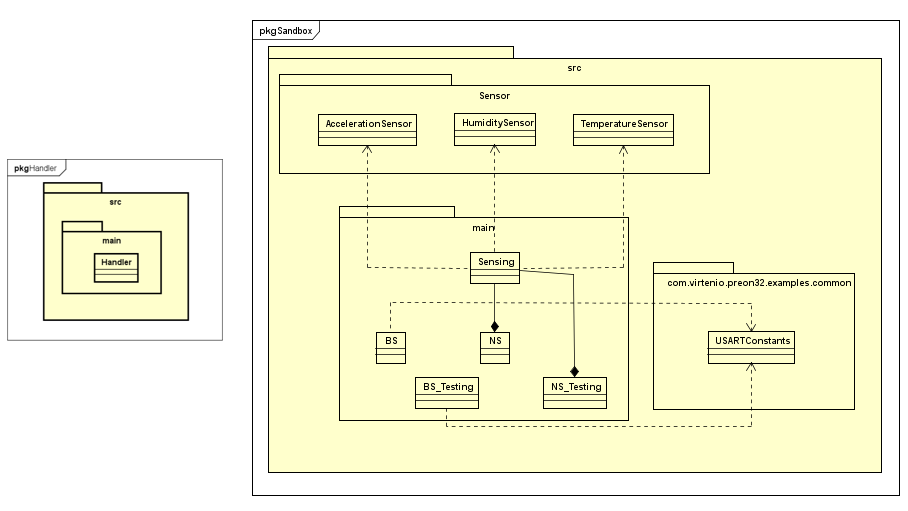
\includegraphics[scale=0.7]{tempsnip}
	\caption{Diagram Kelas Sederhana Dari Aplikasi Transfer Data Pada WSN}
	\label{fig:tempsnip}
\end{figure}
Berikut adalah penjelasan dari kelas-kelas pada diagram di Gambar~\ref{fig:tempsnip}
\begin{itemize}
    \item Package Sensor
    \begin{itemize}
        %\item Kelas PressureSensor\\
        %Kelas ini digunakan untuk melakukan pengukuran tekanan udara pada satu waktu.
        \item Kelas AccelerationSensor\\
        Kelas ini digunakan untuk melakukan pengukuran getaran pada satu waktu.
        \item Kelas HumiditySensor\\
        Kelas ini digunakan untuk melakukan pengukuran kelembaban pada satu waktu.
        \item Kelas TemperatureSensor\\
        Kelas ini digunakan untuk melakukan pengukuran suhu pada satu waktu.
    \end{itemize}
    \item Package main
    \begin{itemize}
        \item Kelas Sensing\\
        Kelas ini menyatukan ketiga buah kelas sensor dan digunakan pada kelas NodeSensor.
        \item Kelas BS\\
        Kelas ini menangani fungsi-fungsi yang ada pada \textit{base station} seperti mengirimkan perintah-perintah kepada node sensor yang terhubung dengan \textit{base station}.
        \item Kelas NS\\
        Kelas ini melakukan \textit{sensing} dan mengirimkan data ke \textit{base station} atau ke node sensor lain.
        \item Kelas BS\_Testing\\
        Kelas ini menangani fungsi-fungsiyang ada pada \textit{base station}. Kelas ini digunakan untuk melakukan pengujian aplikasi yang tidak \textit{reliable}.
        \item Kelas NS\_Testing\\
        Kelas ini melakukan \textit{sensing} dan mengirimkan data ke \textit{base station} atau ke node sensor lain. Kelas ini digunakan untuk melakukan pengujian aplikasi yang tidak \textit{reliable}.
    \end{itemize}
    \item Package handler
    \begin{itemize}
        \item Kelas handler\\
        Kelas yang digunakan untuk menangani semua interaksi antara pengguna dengan Base Station.
    \end{itemize}
    \item Package com.virtenio.preon32.example.common
    \begin{itemize}
        \item Kelas USARTConstants\\
        Kelas yang digunakan untuk membuat koneksi antara \textit{base station} dengan program pada komputer pengguna.
    \end{itemize}
\end{itemize}

\subsection{Fitur dan Kebutuhkan Sistem}
\label{subsec:fitur_dan_kebutuhan_sistem}
Pada subbab ini dijelaskan fitur-fitur dan kebutuhan sistem dalam membangun aplikasi transfer data yang \textit{reliable} di WSN.

\subsubsection{Arsitektur Flat}
Pada arsitektur flat tidak terdapat hierarki dan \textit{cluster head}. Setiap node sensor yang telah melakukan \textit{sensing} akan mengirimkan data dengan cara meneruskan data ke node sensor tetangganya. Node sensor tetangganya tersebut yang akan meneruskan data ke node sensor lain hingga sampai ke \textit{base station}. Beberapa contoh arsitektur flat dapat dilihat pada Gambar~\ref{fig:contoh_flat}.
\begin{figure}[htbp]
	\centering
	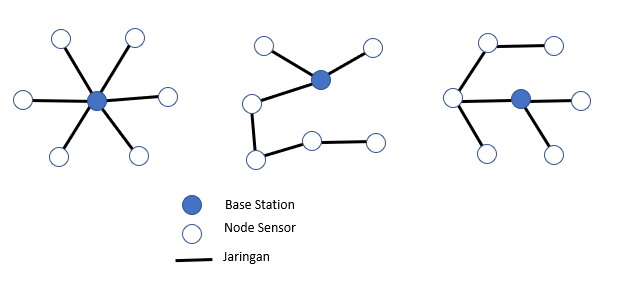
\includegraphics[scale=0.7]{contoh_flat}
	\caption{Contoh arsitketur flat}
	\label{fig:contoh_flat}
\end{figure}

Gambar \ref{fig:flowchart} adalah \textit{flowchart} dalam melakukan transfer data pada arsitektur flat dan cara menangani data yang hilang.

\begin{figure}[htbp]
	\centering
	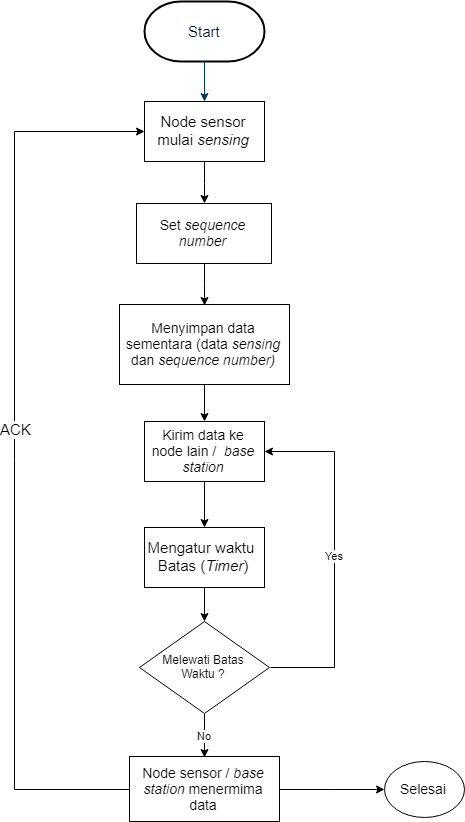
\includegraphics[scale=0.5]{flowchart}
	\caption{Flowchart transfer data dengan ACK dan \textit{timer}}
	\label{fig:flowchart}
\end{figure}

Berikut adalah penjelasan dari Gambar \ref{fig:flowchart}.
\begin{enumerate}
	\item Node sensor melakukan \textit{sensing}.
	\item Disaat yang bersamaan node sensor menetapkan waktu \textit{timer} untuk data yang akan dikirim.
	\item Node sensor mendapatkan data-data hasil \textit{sensing}.
	\item Data yang didapat ini berisi \textit{sequence number}, \textit{timestamp} dan data utama hasil \textit{sensing}.
	\item Data disimpan sementara dan diteruskan ke node sensor tetangganya.
	\item Node sensor(\textit{receiver}) yang menerima data dari node sensor sebelumnya (\textit{source}) akan meneruskan data tersebut ke node lain hingga sampai ke \textit{base station}.
	\item Jika data sudah sampai ke \textit{base station}, \textit{base station} akan mengirimkan ACK ke node yang terhubung dengan \textit{base station}.
	\item ACK akan diteruskan ke node lain jika tidak sesuai dengan pengirim data \textit{sensing} tersebut.
	\item Saat node sensor pengirim data menerima ACK, node sensor tersebut akan melakukan \textit{sensing} lagi.
	\item Jika sudah melewati batas waktu \textit{timer}, node sensor akan mengirimkan ulang data yang sudah tersimpan.
\end{enumerate}

\subsubsection{Routing Pada Aplikasi Transfer Data}
\label{subsec:routing}
Untuk melakukan monitoring area, node sensor mengirimkan data langsung kepada \textit{base station} atau melalui node sensor lain hingga sampai \textit{base station}. Dalam mengirimkan data diperlukan alamat tujuan data akan dikirimkan. Pada \textit{single-hop} pertukaran data hanya antara node sensor dengan \textit{base station}, sedangkan pada \textit{multi-hop} data akan diteruskan kepada node sensor beberapa kali hingga sampai kepada alamat yang dituju. 

Aplikasi yang dibangun akan menyimpan alamat \textit{base station} itu sendiri dan alamat node lain. Pada \textit{base station} menyimpan alamat dirinya dan juga alamat node-node yang terhubung langsung dengan \textit{base station}. Sedangkan pada node sensor menyimpan alamat node sensor tersebut, alamat tujuan untuk mengirimkan data hasil \textit{sensing} dan alamat node sensor lain untuk mengirimkan perintah-perintah. Sehingga untuk mengirimkan data hasil \textit{sensing}, node sensor akan mengirimkan kepada 1 tujuan (\textit{unicast}). Sedangkan untuk mengirimkan perintah, node sensor dapat mengirimkan kepada banyak node sensor lain secara \textit{multicast}.

\subsection{Ukuran Reliability}
Pada aplikasi yang dibangun, setiap node sensor akan melakukan \textit{sensing} secara terus menerus hingga pengguna menghentikan program. Node sensor akan berhenti jika menerima perintah berhenti dari \textit{base station}. Data yang didapat ini yang akan dikirimkan ke \textit{base station} dan digunakan untuk monitoring.

Setiap data yang dikirim memiliki \textit{sequence number}. \textit{Sequence number} ini yang akan menjadi perhitungan untuk memastikan \textit{reliability}. Pengguna melihat keterurutan dari \textit{sequence number} setiap data yang telah diterima oleh \textit{base station}. Jika didapat \textit{sequence number} dengan urut, maka \textit{reliability} pada aplikasi ini berhasil.

\section{Analisis Proses Pengiriman Data Dari Node Sensor Ke Base Station Pada WSN}
Pengiriman data pada WSN dibagi menjadi dua yaitu pengiriman data dari \textit{base station} ke setiap node sensor (\textit{downstream}) dan pengiriman data dari setiap node sensor ke \textit{base station} (\textit{upstream}). Pengiriman \textit{downstream} biasanya adalah perintah yang diberikan oleh \textit{base station} kepada node sensor, sedangkan pengiriman \textit{upstream} adalah pengiriman data hasil \textit{sensing} setiap node sensor kepada \textit{base station}. 

Pengiriman data hasil \textit{sensing} dari node sensor ke \textit{base station} sendiri dapat dilakukan dengan dua cara yaitu setiap data hasil \textit{sensing} langsung dikirimkan ke \textit{base station} tanpa melalui proses apapun pada node sensor dan data hasil \textit{sensing} diproses dahulu pada node sensor lalu dikirimkan. Kedua cara ini sebenarnya dapat digunakan sesuai dengan kebutuhkan dan kapasitas penyimpanan pada node sensor. Pada umumnya node sensor memiliki tempat penyimpanan yang kecil, sehingga kode program yang dibuat tidak dapat terlalu besar dan data hasil \textit{sensing} harus dikelola saat akan melakukan pengiriman.

Pada skripsi ini, aplikasi yang dibangun adalah aplikasi transfer data yang \textit{reliable}. Sehingga data yang dikirim harus dikelola dahulu. Sedangkan untuk membuktikan aplikasi \textit{reliable} ini berhasil, dibuat juga aplikasi yang tidak \textit{reliable} sebagai perbandingan data yang diterima. Untuk aplikasi yang tidak \textit{reliable} ini data yang dikirimkan adalah data mentah hasil \textit{sensing}.

\subsection{Format Pesan Yang Dikirim}
\label{sub:formatPesan}
Setelah sensor mendapatkan data \textit{sensing} dari lingkungannya, perlu ditentukan bagaimana format data yang akan dikirimkan ke node sensor lain. Data hasil \textit{sensing} ini akan dikirim melalui \textit{frame}. Setiap \textit{frame} memiliki batasan panjang data yang bisa dikirimkan (PHY Payload). Untuk setiap data ada beberapa hal penting yang perlu ada untuk mendukung transfer data yang \textit{reliable}, yaitu:
\begin{enumerate}
    \item \textit{Sequence number}.
    \item \textit{Timestamp}.
    \item Data utama.
\end{enumerate}
 
\textbf{\textit{Sequence number}} digunakan untuk menentukan urutan pengiriman data dari node sensor ke node sensor lain. Data yang \textit{loss} dapat dilihat dari \textit{sequence number} ini. \textbf{\textit{Timestamp}} digunakan untuk menentukan kapan waktu data diambil. \textbf{Data utama} adalah data hasil \textit{sensing} yang diperoleh dari setiap sensor.

Untuk memastikan data yang diterima telah sampai ke \textit{base station}, maka \textit{base station} harus melakukan pengiriman ACK kepada node sensor yang melakukan \textit{sensing}. ACK ini juga dimaksudkan untuk mengatur ulang waktu \textit{timer} pada node sensor. Untuk setiap pesan ACK yang dikirimkan ada beberapa hal penting yang perlu ada untuk mendukung transfer data yang \textit{reliable}, yaitu:
\begin{enumerate}
    \item Pesan "ACK".
    \item Alamat node sensor sumber data.
    \item \textit{Sequence number} dari data yang diterima.
\end{enumerate}

\textbf{Pesan "ACK"} digunakan untuk menandakan bahwa pesan yang dikirim dari \textit{base station} kepada node sensor adalah ACK. Pesan "ACK" ini akan diikuti dengan \textbf{\textit{alamat node sensor sumber data}}. Dari \textit{base station} pesan ini akan dikirimkan kepada node sensor yang terhubung kepada \textit{base station}, saat node sensor menerima pesan ini dan alamat node sensor pada pesan tersebut bukan alamat node sensor penerima, maka pesan tersebut akan diteruskan kepada node sensor lain yang terhubung. Setelah alamat node sensor, pesan akan diikuti dengan \textbf{\textit{sequence number}}. \textit{Sequence number} digunakan node sensor untuk mengetahui apakah pesan yang diterima \textit{base station} sama dengan pesan yang node sensor kirim.

\section{Analisis Protokol Transfer Yang Reliable Pada WSN Untuk Digunakan Dalam Membangun Aplikasi Transfer Data}
Tidak semua protokol pengiriman data pada WSN mendukung pengiriman data yang \textit{reliable}. Pada WSN terdapat beberapa protokol yang mendukung pengiriman data reliable. Untuk memastikan data yang \textit{reliable} ini dilakukanlah pengiriman ulang (\textit{retransmission}) data yang hilang atau \textit{loss}. Data yang dikirim ulang ini dapat berasal dari hasil \textit{sensing} node sensor atau data dari \textit{base station} seperti perintah atau \textit{method} untuk melakukan sesuatu. Pada skripsi ini data yang dikirim ulang adalah data hasil \textit{sensing} sehingga protokol yang digunakan adalah protokol dengan arah pengiriman \textit{upstream}. Setiap protokol memiliki spesifikasi yang berbeda-beda pada arah \textit{retransmission}, data yang dikirim, dan mekanisme \textit{acknowledge} yang digunakan. Data yang diperoleh node sensor ini dapat diteruskan ke node sensor tetangganya dahulu sebelum sampai ke tujuan akhir yaitu \textit{base station} (\textit{multihop}). 

Aplikasi transfer data yang dibangun ini mengadaptasi beberapa cara yang terdapat pada protokol RMST untuk menangani \textit{reliability} transfer data dari node sensor ke \textit{base station}. RMST dapat melakukan \textit{retransmission} dengan mekanisme \textit{hop-by-hop} dan \textit{end-to-end} \cite{rmst}. Aplikasi dibangun menggunakan mekanisme \textit{end-to-end} dengan bantuan ACK dalam memastikan data sampai \textit{base station}. Dengan mekanisme \textit{end-to-end}, node sensor akan mengirimkan data ke node tetangga dan diteruskan ke node sensor lain hingga sampai di \textit{base station}. Setelah \textit{base station} mendapatkan data hasil \textit{sensing}, \textit{base station} akan mengirimkan ACK kepada node sensor di bawahnya dan diteruskan hingga sampai kepada node sensor pengirim data tersebut. Node sensor yang sedang mengirim data akan menunggu ACK yang didapat dari node di atasnya.

Protokol RMST ini juga menggunakan \textit{timer-driven}. Mekanisme \textit{timer-driven} ini adalah batas waktu menunggu ACK atau NACK untuk dilakukan pengiriman ulang. Pada aplikasi yang dibangun juga menggunakan mekanisme \textit{timer-driver}. Saat node sensor telah mengirimkan data, node sensor tersebut akan mengatur (\textit{timer}) atau batas waktu menunggu. Jika sudah melewati batas waktu, maka node sensor akan mengirimkan ulang data kepada node sensor tujuan. Saat melakukan pengiriman ulang data, dapat terjadi duplikasi data yang pada \textit{base station}. Jika ini terjadi maka digunakan \textit{sequence number} untuk memastikan urutan data. Saat data yang diterima memiliki \textit{sequence number} yang sama dengan dengan sebelumnya, maka data tidak akan disimpan.

